\documentclass{interim}
\usepackage{physics, amssymb, graphicx, fancyvrb}
\usepackage[colorlinks=true, allcolors=blue]{hyperref}
\usepackage{pdfpages}

% alternative font if you prefer
% \usepackage{times}

% for alternative page numbering use the following package
% and see documentation for commands
%\usepackage{fancyheadings}


% other potentially useful packagess
% \uspackage{amssymb,amsmath}
% \usepackage{url}
% \usepackage{fancyvrb}
% \usepackage[final]{pdfpages}

\begin{document}

%%%%%%%%%%%%%%%%%%%%%%%%%%%%%%%%%%%%%%%%%%%%%%%%%%%%%%%%%%%%%%%%%%%
\title{3D Face Recognition from RGB Camera and Radar Sensor}
\author{Stergious Aji}
\date{\today}
\maketitle
%%%%%%%%%%%%%%%%%%%%%%%%%%%%%%%%%%%%%%%%%%%%%%%%%%%%%%%%%%%%%%%%%%%

%%%%%%%%%%%%%%%%%%%%%%%%%%%%%%%%%%%%%%%%%%%%%%%%%%%%%%%%%%%%%%%%%%%
{\hypersetup{hidelinks}\tableofcontents}
\newpage
%%%%%%%%%%%%%%%%%%%%%%%%%%%%%%%%%%%%%%%%%%%%%%%%%%%%%%%%%%%%%%%%%%%

%%%%%%%%%%%%%%%%%%%%%%%%%%%%%%%%%%%%%%%%%%%%%%%%%%%%%%%%%%%%%%%%%%%
\section{Introduction}\label{intro}
% briefly explain the context of the project problem
% Please note your proposal need not follow the included section headings - this is only a suggested structure. Also add subsections etc as required
% example references: \cite{BK08}

\subsection{Motivation}
Facial recognition technology is a crucial field of research due to its broad applications in areas such as security surveillance, forensic analysis, human-computer interaction, and healthcare. Its most notable use is in biometric authentication for access control. This enables a non-invasive, hands-free approach to identity verification, removing the need to remember passwords. Furthermore, facial biometrics are naturally more accessible than other forms such as fingerprints, iris, or palm prints.

Since its inception in the 1960s, face recognition systems have evolved significantly. The pioneering work by Bledsoe \cite{bledsoe1966model} distinguished faces by comparing distances of manually annotated landmark features such as the nose, eyes, and mouth. In more recent years, the advent of Deep Learning has greatly improved the performance of human face classification, benefiting from the vast online database of face images.  However, these systems primarily rely on 2D images from RGB cameras making them susceptible to variations in lighting and pose. To compensate for this, the depth information of facial attributes is essential. Additionally, transitioning to 3D facial recognition not only improves accuracy but also enhances the security of biometric systems.

The popularity of 3D face recognition is on the rise, evidenced by its adoption in smartphones with the likes of Apple's Face ID \cite{apple-faceid}. This growing demand has pushed the miniaturisation of depth-sensing technology to smaller form factors, enabling it to operate efficiently in real-time on mobile devices with minimal computational power. Depth cameras used in this context typically employ an active face acquisition method, where non-visible light is projected onto the face and reflected back, allowing sensors to measure and map facial features. The most common approach uses Lidar, emitting waves in the Near-Infrared spectrum, due to its ability to capture a dense 3D map of the subject face. However, its weakness in penetrating materials like clothing and hair is a notable limitation. In contrast, millimetre Radar waves can penetrate such obstacles to directly reach the dermal layer of the skin \cite{vizard2006advances}, potentially offering better performance in occlusion scenarios or even within the presence of rain or fog.

Research into the efficacy of Radar waves for 3D face recognition is relatively sparse but recent existing studies show positive results \cite{hof2020face, lim2020dnn,kim2020face, pho2021radar,challa2021face}. Radar technology is generally more cost-effective, both in terms of acquisition and computationally since it consumes less power compared to Lidar cameras. However, the lower accuracy and sparsity of mmWave signatures may hinder its effectiveness in facial recognition. A solution is to integrate RGB information with the depth data obtained by Radar sensors to enhance the system's ability to accurately learn and identify facial characteristics.


\subsection{Aims}
This project aims to explore the effectiveness of using RGB cameras in conjunction with mmWave Radar sensors for 3D facial recognition. Since there are no appropriate datasets available for this purpose, we will be required to collate this data ourselves. We plan to use the Intel RealSense L515 camera \cite{intel-l515} for capturing RGB images of an individual's face. The Google Soli Radar sensor \cite{lien2016soli} will be employed to gather depth data through reflected millimetre waves. 

Given the necessity of data collection, our goal is to gather facial data from approximately 50 participants. This number is expected to be sufficient for both training and evaluating our proposed model within the limited timeframe. We aim to obtain face data under various conditions including different poses, lighting environments, and common occlusion scenarios. The objective is to empirically validate the benefits of utilising mmWave technology in this context. We hypothesise that this approach would yield a system that is invariant to pose, lighting, and occlusion compared to using RGB or depth information individually.

Next, we plan to develop a novel face recognition model using a Deep Convolutional Neural Network. This model will be trained on the captured facial data in order to learn facial features from both the RGB and depth information acquired from the Soli sensor. We intend to investigate different data fusion techniques to identify the most effective strategy that provides a rich and distinctive facial representation for accurate classification performance. 

% This RealSense camera also includes a LiDAR sensor which produces a more accurate dense depth image. As a backup, a separate model can be trained to transform the sparse Soli data into a more dense representation before inputting into the facial recognition model. However, if the Radar data works well this may not be needed. (MAY NOT INCLUDE)

%%%%%%%%%%%%%%%%%%%%%%%%%%%%%%%%%%%%%%%%%%%%%%%%%%%%%%%%%%%%%%%%%%%
% \section{Statement of Problem??}

% clearly state the problem to be addressed in your forthcoming project. Explain why it would be worthwhile to solve this problem.

%%%%%%%%%%%%%%%%%%%%%%%%%%%%%%%%%%%%%%%%%%%%%%%%%%%%%%%%%%%%%%%%%%%
\section{Background Survey}
% present an overview of relevant previous work including articles, books, and existing software products. Critically evaluate the strengths and weaknesses of the previous work.
Before any work is conducted, a review of relevant literature in the field is undertaken. This is essential to corroborating best practices and gaining a deeper insight of the strengths and limitations of mmWave Radar sensors, in the context of face recognition. Next, a look into existing datasets compatible with our research objectives is performed, followed by a detailed justification for the need to compile our own dataset. Furthermore, an analysis of the recent work with Radar technology specifically for the purpose of human face classification is provided.

\subsection{mmWave Radar Technology}
Radio Detection and Ranging, or RADAR, has been around for decades and is instrumental in fields such as space exploration, military and commercial aviation, maritime navigation, as well as, meteorology. Recently, the miniaturisation of Radar sensors to the millimetre wave (mmWave) band has brought its application to more small-scale domains \cite{soumya2023recent}. A notable example is Google's integration of the Soli sensor into their Pixel 4 smartphone for facial detection and motion gesture recognition \cite{googleblog2020}. This is the exact sensor we plan to utilise during this project's data collection phase. A key driving factor for this choice is the Soli's use of Frequency Modulated Continuous Wave (FMCW) technology. This is proven to offer superior range resolution in comparison to other modulation techniques due to its high pulse compression \cite{mahafza2005radar}, a vital aspect for generating accurate facial embeddings. 

mmWave sensing is also being explored in the domain of autonomous vehicles, specifically in systems such as collision warnings and adaptive cruise control \cite{dfrobot}. This is primarily due to its edge over traditional Near-Infrared waves employed by Light Detection and Ranging (LiDAR) cameras, particularly in its resilience against atmospheric conditions such as dust, smoke, fog, and rain \cite{cadenceblog2022}. This penetrative power of mmWaves makes it a promising candidate for reliable facial recognition in diverse, real-world scenarios. However, it is important to note the trade-off as mmWaves tend to have lower accuracy in comparison, which could impact 3D facial recognition performance where precision in detecting and mapping facial features is paramount. This project will therefore explore counter-balancing this limitation with the information gained from RGB images, potentially paving the way for more resilient and versatile systems.


\subsection{Data Acquisition}
\label{background:data_acquisition}
Various methods exist for capturing 3D face data which can be broadly categorised into two main types: \textit{Active} and \textit{Passive} techniques \cite{zhou20183d}. Active systems emit non-visible light onto the target and use the reflected light to construct a 3D point cloud of the subject. Contrastingly, passive systems rely on the available light in the scene to capture facial features. For instance, stereoscopic cameras use two or more cameras to capture images of the subject from different perspectives to enable depth perception. In addition, 3D facial features can be inferred using shape-from-shading techniques which analyse the luminance values contained in 2D grayscale images \cite{horn1977understanding}.

Passive systems, advantageous for their ability to operate in real-time without light emission, are highly influenced by environmental lighting conditions. Active systems, in contrast, are more robust as they use their own light to illuminate the subject, permitting functionality even in dimly lit settings. Active acquisition often involves structured light and triangulation methods to gather depth information. In the case of Lidar cameras like the Intel RealSense, the time-of-flight of emitted light is measured to gauge the distances of points on the target. The Soli sensor is another form of active acquisition, using three receiving antennas to capture reflected mmWaves, measuring the phase difference and Doppler shift to estimate the distance and radial velocity of the target. 

When collecting data on human faces for 3D face recognition, it is crucial to ensure the data comprises a wide range of facial poses, expressions, lighting conditions and occlusion scenarios. Unlike 2D images, the pure geometric information from 3D face scans ensures that models are insensitive to pose and lighting changes during training. Research by \cite{prabhu2011unconstrained} found that the maximum pose angle that their Local Binary Pattern-based model is robust against is $60^\circ$. Additionally, a diverse range of genders, ages, and ethnicities is essential for real-world applicability.

In recent years, the number of 3D face databases available has grown, encompassing various acquisition techniques and devices. Noteworthy datasets include the BU-3DFE \cite{yin20063d} and the FRGC \cite{phillips2005overview} database, widely accepted as standard references for evaluating the performance of 3D face recognition systems. The BU-3DFE dataset, focusing on expression variance, contains six types of expressions from 100 individuals, captured using stereo photography. While these datasets are unsuitable for our project, the data collection procedure used to amass them provides valuable insights. Presently, there is only one public database featuring Radar signatures of 206 human faces \cite{mmwavefacedata}. This dataset was captured with a Qualcomm 60 GHz mmWave Radar, however, lacks any RGB face images of the participants in the study. These factors motivate building our own dataset including both RGB images and mmWave Radar face signatures. This also enables flexibility to tailor our experiment design to investigate the model's effectiveness under specific conditions such as lighting and pose variations, and occlusion.


\subsection{Prior Work on Radar-based Face Recognition}
The use of mmWaves for human face identification is a relatively new research field driven by the advancement of Radar sensor technology to the millimetre wave band. One of the earliest papers found to investigate human identification using mmWaves dates back to 2019 \cite{zhao2019mid}. While this paper focuses on the simultaneous classification of people by their gait and body shape rather than facial features, it displayed the ability of mmWaves to capture subtle idiosyncrasies among individuals. These nuanced differences are crucial for learning models to effectively distinguish between people, leading to high classification accuracies.

Following this, Hof et al. \cite{hof2020face} proposed a Deep Neural Network (DNN) based Autoencoder that is able to distinguish human faces captured by an 802.11ad/y networking chipset operating at a centre frequency of 60 GHz. The Autoencoder is able to encode mmWave face signatures of over 200 individuals with enough separation to distinguish positive and negative instances by measuring their Mean Squared Error (MSE) against reference facial embedding. The study conducted an extensive data collection process, capturing mmWave signatures of 206 individuals of varying genders and ages, in five different poses: frontal, as well as, $15^\circ$ and $25^\circ$ rotations to the left and right. This dataset was subsequently made available through an IEEE Data Port \cite{mmwavefacedata}. While this dataset encapsulates faces from a wide range of people, including some with beards and spectacles, it lacks representation of other common occlusion scenarios like head accessories, that our project aims to explore. Moreover, the study utilised a large sensor containing 1024 transmitting and receiving antenna pairs. This is in contrast to the compact Soli chip with a single transmit and three receiver antennas, intended to work in a smartphone. Notably, the study simulated the effect of reducing the antenna count to 10, markedly decreasing the distinctiveness of facial signatures. Promisingly, increasing the number of neurons in their Neural Network and an additional hidden layer could compensate for this reduction, maintaining high accuracy.

Lim et al. \cite{lim2020dnn} also proposed another Deep Neural Network model, however with a more representative Multi-Layer Perceptron (MLP) architecture where every layer is fully connected to adjacent layers. The study utilised a small-scale 61 GHz FMCW Radar sensor by bitsensing Inc. \cite{bitsensing2020bts60}, comparable to the Google Soli with a single transmit and 3 receiver antennas. The model attained a mean classification accuracy of 92\% across eight subjects. The study also showed that their DNN approach surpassed the performance of both a Support Vector Machine (SVM) and tree-based Ensemble Learning approaches, trained on the same mmWave facial features. It is important to note the relatively small-sized dataset used to train the model raising concerns about potential overfitting as the data is not representative enough. The paper provides limited details on the data collection methodology used, only mentioning that the facial distances ranged from 30 cm to 50 cm. It can be assumed that the study likely focussed on front facial poses without any occlusions for all eight subjects. The research also explored the impact of using a single receiving antenna, which resulted in a reduced accuracy of 73.7\%. This finding is in line with Hof et al.'s \cite{hof2020face} observation that an increased number of receiving antennas can enhance classification accuracy by capturing more nuanced facial features. The paper also suggests that a CNN may be more appropriate if signals were stacked on the time axis rather than the frequency axis.

During the same period, Kim et al. \cite{kim2020face} conducted research using the same 61 GHz FMCW Radar sensor from bitsensing Inc., featuring a range resolution of 2.5 cm. Their study introduced a CNN model composed of three convolutional layers and three fully connected layers. The radar data underwent heavy preprocessing to transform it into a more image-like format suitable for the CNN model. With a data split of 70\%/15\%/15\% for training, validation, and testing, the model achieved an average classification accuracy of 98.7\% on a limited dataset of only three individuals. Interestingly, the study also examined the impact of wearing cotton masks. The results showed a minimal drop in average classification accuracy by 0.9\%, which is encouraging for the objectives of our project. However, these findings are taken with caution due to the small scale of the dataset. It remains unclear whether this level of performance would hold consistently across a larger and more diverse group of subjects and with more varied occlusions.

Pho et al. \cite{pho2021radar} adopts a One-Shot Learning approach to the problem. This is where a model is trained with a single or only a few labelled instances. This is beneficial when there is a lack of training samples available. The proposed method constitutes a Siamese structure of two identical CNNs with shared parameters that map the input Radar signals into the embedding space. A distance metric between the outputs of both CNNs are used in training and testing to measure the similarity of facial inputs. The model is trained for \textit{binary classification} by inputting pairs of face signatures from either the same or different people. This process aims to learn embeddings that push different faces into distinct Euclidean regions of the embedding space. The same bitsensing Inc. BTS60 chipset, used by \cite{lim2020dnn, kim2020face}, was employed to capture 500 frames of the faces of eight participants. An average classification of 97.6\% was achieved, an improvement from the previous DNN model by Lim et al. \cite{lim2020dnn} with the same number of people. t-Stochastic Neighbour Embedding (t-SNE) \cite{van2008visualizing} was applied for dimensionality reduction. The resulting visualisations demonstrated that the one-shot Siamese network effectively distinguished each individual's face, simplifying the classification task. While a small dataset is used only encompassing frontal poses with no occlusion, the proposed method is well documented and is likely robust against larger datasets.

Challa et al. \cite{challa2021face} employs two different machine learning models on the dataset made available at \cite{mmwavefacedata}. Their approach began with a CNN-based Autoencoder followed by a Random Forest Ensemble Learning approach. A total of nine Autoencoders are built, each tailored to different frame rates, focusing on compressing and learning to reconstruct the original data from its compressed, latent form. The Autoencoders are trained using randomly selected data samples from 186 mmWave face signatures from the data port. The flattened and labelled outputs are then used to train and test nine discrete Random Forest models using identical hyperparameters, as recommended by the Sci-kit library. This methodology yielded impressive results, achieving an average classification accuracy of 99.98\% using all 1400 frames per individual. Even reducing the number of frames to 70 per person, the model maintained a high accuracy of 97.1\%. The paper presents an approach that is unique in comparison to the rest of the research papers tackling this subject, showcasing a model that is able to be deployed on mobile chips.

The research in this area primarily focuses on utilising data exclusively from Radar sensors, largely driven by concerns for privacy preservation. However, a significant limitation of this approach is the required duration for capturing an accurate facial scan. The sensor needs to operate for several seconds, typically in the range 10 to 15 seconds, to obtain a detailed scan. Such a time frame is impractical in real-world situations, as it necessitates the subject to remain motionless for a prolonged period. Up to this point, no study has explored the potential benefits of combining Radar signatures with corresponding RGB data to enhance facial recognition capabilities. Given the high performance of existing deep learning models using 2D RGB data alone, such as InsightFace \cite{deng2018arcface}, integrating these models with mmWave Radar data presents a promising avenue. This combination could accelerate data acquisition while leveraging the advantages of mmWaves in terms of their robustness to lighting variations and occlusions.


\subsection{InsightFace}
\label{background:insightface}
In the evolving field of face recognition, deep CNNs have emerged as a dominant approach due to their ability to extract rich, discriminative facial features from images. One significant advancement in this area is the InsightFace toolkit, implementing algorithms designed to address the intricacies of face analysis and recognition. Key works include the preliminary ArcFace model, introduced by Deng et al. \cite{deng2018arcface}, alongside the robust Face Alignment model by Gho et al. \cite{guo2018stacked}. ArcFace employs a novel Additive Angular Margin Loss to maximize class separability, further enhancing the discriminative power in mapping 2D facial images to feature embeddings. However, this method was found to face challenges with label noise, requiring the "cleaning" of many real-world images sourced from the web. To address this, further progress was made with Sub-center ArcFace \cite{deng2020subcenter}, introducing the concept of sub-classes to boost resilience against intra-class variations and label noise. It achieved state-of-the-art performance on many widely used benchmark datasets such as the Labeled Faces in the Wild (LFW) \cite{huang2008labeled} and YouTube Faces (YTF) datasets \cite{wolf2011face}.

The integration of pretrained models offered by InsightFace into our system enables us to concentrate primarily on enhancing the performance of our CNN embedding mmWave face signatures. By fusing the depth and contour detection capabilities of mmWave Radar with the rich textural features gathered by ArcFace from RGB images, the system has the potential to attain improved accuracy and robustness. This approach is particularly promising in environments where conventional optical methods falter.


\subsection{Multimodal Data Fusion Techniques}
\label{background:multimodal_data_fusion_techniques}
Multimodality, as defined by Lahat et al. \cite{lahat2015multimodal}, refers to the use and analysis of multiple types of data, potentially arriving from multiple sensors. The aim is to extract and blend salient information gathered by each sensor. The integration of this diverse data leads to outputs with richer representation and performance than what could be achieved by individual modalities alone. We hypothesise that coupling the colour information from face images with the depth gathered by the Radar sensor could greatly improve class separation, and subsequently, face recognition performance.

A common technique involves fusing the multiple data modalities before feeding them into a learning model, referred to as \textbf{Early Fusion}, or \textbf{Data Level Fusion}. It includes combining data by removing correlations between sensors or fusing data in a common, lower-dimensional space. Techniques such as Principal Component Analysis (PCA) and Canonical Correlation Analysis (CCA) are commonly employed for this purpose. One key issue with early fusion is ensuring synchronisation between the RGB and Radar frames, which is difficult due to their significantly different sampling rates. Furthermore, the continuous mmWave signals must be effectively discretised to match the form of the RGB data. A major disadvantage of early fusion is the potential to squash critical information present within each individual modality, impacting the training efficacy.

\textbf{Late Fusion}, or \textbf{Decision Level Fusion}, operates by independently processing different data sources through separate models and then fusing them at the decision-making stage. A common approach involves taking a weighted average of the separate predictions, providing a way to minimise or maximise the influence of specific modalities. Late Fusion is often simpler and flexible, and can be very effective when dealing with extremely dissimilar data sources either in terms of sampling rate, dimensionality, or unit of measurement. Additionally, late fusion often yields better performance since errors from multiple models are dealt with independently.

\textbf{Intermediate Fusion} or \textbf{Feature Level Fusion} is based on DNN architectures and is the idea of combining different modalities in the feature space where there is a higher level of abstraction of the raw data. This can be as straightforward as a simple concatenation of the individual latent embeddings or utilising Autoencoders for non-linear feature fusion \cite{charte2018practical}. This approach offers greater versatility than early and late fusions, as it allows for the integration of features at various depths within the neural network. However, it can lead to challenges with a risk of overfitting or the failure in learning relationships between the different modalities.

Each data fusion technique comes with its own set of challenges and considerations, necessitating experimentation to determine the most effective way to merge the RGB and mmWave signatures. A variant of late-intermediate fusion is the most feasible where the embeddings from the last layers of each model is combined. It would be challenging to attempt early fusion due to the substantial differences between the two modalities. Such integration would likely require heavy preprocessing of the Radar data, potentially involving its conversion into a depth image-like format. 


\subsection{Deep Learning for Face Recognition}
The most popular methodology observed for creating face recognition models involve deep learning, specifically through the use of Convolutional Neural Networks (CNN). Before proceeding to develop our own model to learn mmWave face signatures, it is vital to grasp the underlying concepts involved and strategies employed in recent research. This understanding will guide us in identifying the most effective strategy for our project.

CNNs are a class of deep neural networks, most commonly applied to the analysis of image data. Inspired by the structure of the animal visual cortex, they are designed to automatically and adaptively learn spatial hierarchies of features from input images. A typical CNN architecture comprises a sequence of layers, including convolutional layers for feature detection, pooling layers for dimensionality reduction, and fully connected layers for final output processing.

Unlike traditional algorithms, CNNs learn to identify the necessary features for classification directly from the input data, minimising the need for manual feature extraction. This is particularly advantageous in face recognition where nuanced features like edges, textures, and specific parts of the human face need to be identified. CNNs are able to do this using their deep hierarchical layers of abstraction. Lower layers may identify contours and simple textures, while deeper layers can detect more complex features like the shape of the nose, eyes and mouth. The same weights are used across different parts of the input, reducing the number of parameters and thereby the complexity of the model. This makes CNNs particularly memory efficient data with high dimensionality such as the mmWave signatures.

In conclusion, the use of CNNs in face recognition is justified by their ability to automatically learn and generalize from data, their efficiency in handling high-dimensional data, and their robustness against variations in input data. These characteristics make CNNs a powerful tool for developing accurate and efficient face recognition systems.


%%%%%%%%%%%%%%%%%%%%%%%%%%%%%%%%%%%%%%%%%%%%%%%%%%%%%%%%%%%%%%%%%%%
\section{Proposed Approach}
% state how you propose to solve the software development problem. Show that your proposed approach is feasible, but identify any risks.
The following section delineates the planned approach to take on the Radar-based facial recognition problem. Each decision and step will be justified with a premonition of upcoming problems and intricacies that may occur during the project lifecycle.

\subsection{Data Acquisition and Experiments}
Following a thorough research of the field, the next steps involve designing and conducting the data acquisition process necessary to train our proposed model with. These experiments require careful planning since the data collected here directly determines the effectiveness of the resulting model. As found in Section \ref{background:data_acquisition} in the Background, it is vital to compile pose variations of the face in order for the model to learn a comprehensive 3D scan of the individual's face. Furthermore, it imposes pose-invariance into the system as people would not always provide an exact frontal pose to a face recognition system in real-world use-cases. Most studies only focus on variations in the yaw axis since a person is less likely to tilt or pitch their head by a significant angle in comparison to the left and right rotation of the face. For this reason, we will also focus primarily on head rotation in the yaw axis, specifically capturing faces poses of $0^\circ$, and $30^\circ$ and $45^\circ$ to the left and right of the sensors indicated by positive and negative angles. 

Since this experiment aims to explore the benefits of mmWave sensors in the context of face recognition, two different lighting conditions will also be incorporated in the data collection experiments. Namely, regular and dim lighting scenarios. We hypothesise that the mmWave face signatures would be invariant to the environmental lighting due to it using its own active illumination of the target face compared to the RGB camera. Therefore, if the system is able to achieve a higher accuracy using both modalities compared to using the RGB information, it would conclusively show that mmWaves offer robustness against varying lighting conditions.

Finally, we aim to investigate the penetrative power of mmWaves to directly reach the skin through cloth and hair by injecting common occlusion scenarios into our experiments. It would be beneficial if facial recognition systems are robust against common occluding head accessories such as hats, glasses, masks and so on. Currently, individuals would have to take these accessories off in order for the system to thoroughly identify and allow them access to the particular device or area. With mmWaves, we hypothesise that this may not be required since facial features could be captured regardless. This could greatly benefit security surveillance where individuals deliberately obscure their faces to hide their identities. In our experiment, we aim to capture scenarios both with and without occlusion, however, differing from the study by Kim et al. \cite{kim2020face} using cotton masks since this is already done, common items like hats, sunglasses and scarves would be used to mirror day-to-day scenarios.

On top of investigating environmental invariances, our study also aims to look at the minimal amount of Radar data required to still yield accurate classifications. Previous work are observed to capture 200 to 2,000 frames which depending on the sampling rate, requires running the sensor for eight seconds and a maximum of 80 seconds for each scenario. This is due to the lower accuracy of mmWaves requiring a longer exposure to provide a dense enough representation. Nevertheless, this is a prolonged amount of time for an individual to keep their face still for. However, since our model will utilise the extra RGB information, this may mean that only a few seconds of Radar frames are needed to still identify the individual. For this reason, all scenarios in our experiment will involve capturing 10 RGB frames and a maximum of 250 frames worth of mmWave bursts which maps to running the Google Soli for 10 seconds at a sampling rate of 25 Hz. This allows investigation of the minimal number of mmWave frames required.

In order to gather a wide variety of faces, we aim to gather 50 participants given the tight timeframe of this project. Following ethical guidelines of sensitive personal information, the participants will comprise of adults mainly university students. However, this over-representation of adults aged 20--25 should not impact our study since age invariance is not something that is being investigated. A total of 15 scenarios will be captured for each participant, each running the sensors for 10 seconds resulting in 150 RGB frames and 3,750 mmWave frames.


\subsection{Proposed Model and \textit{mmFace}}
Following the research done in Section \ref{background:insightface} in the Background chapter, it is clear that the ArcFace model available in the InsightFace toolkit is the best choice for this project. It achieves state-of-the-art classification results, outperforming the previous bests such as Facebook's DeepFace \cite{taigman2014deepface} and Google's FaceNet \cite{schroff2015facenet}. This allows treating the handling of the RGB data with a black-box model and a focus on perfecting the Radar-based model we are naming \textit{mmFace}. Furthermore, this enables exploration into the various ways in fusing the two modalities as discussed in Section \ref{background:multimodal_data_fusion_techniques}. Figure \ref{fig:model_architecture} shows a high-level plan of the model architecture described here.

\begin{figure}[h!]
    \centering
    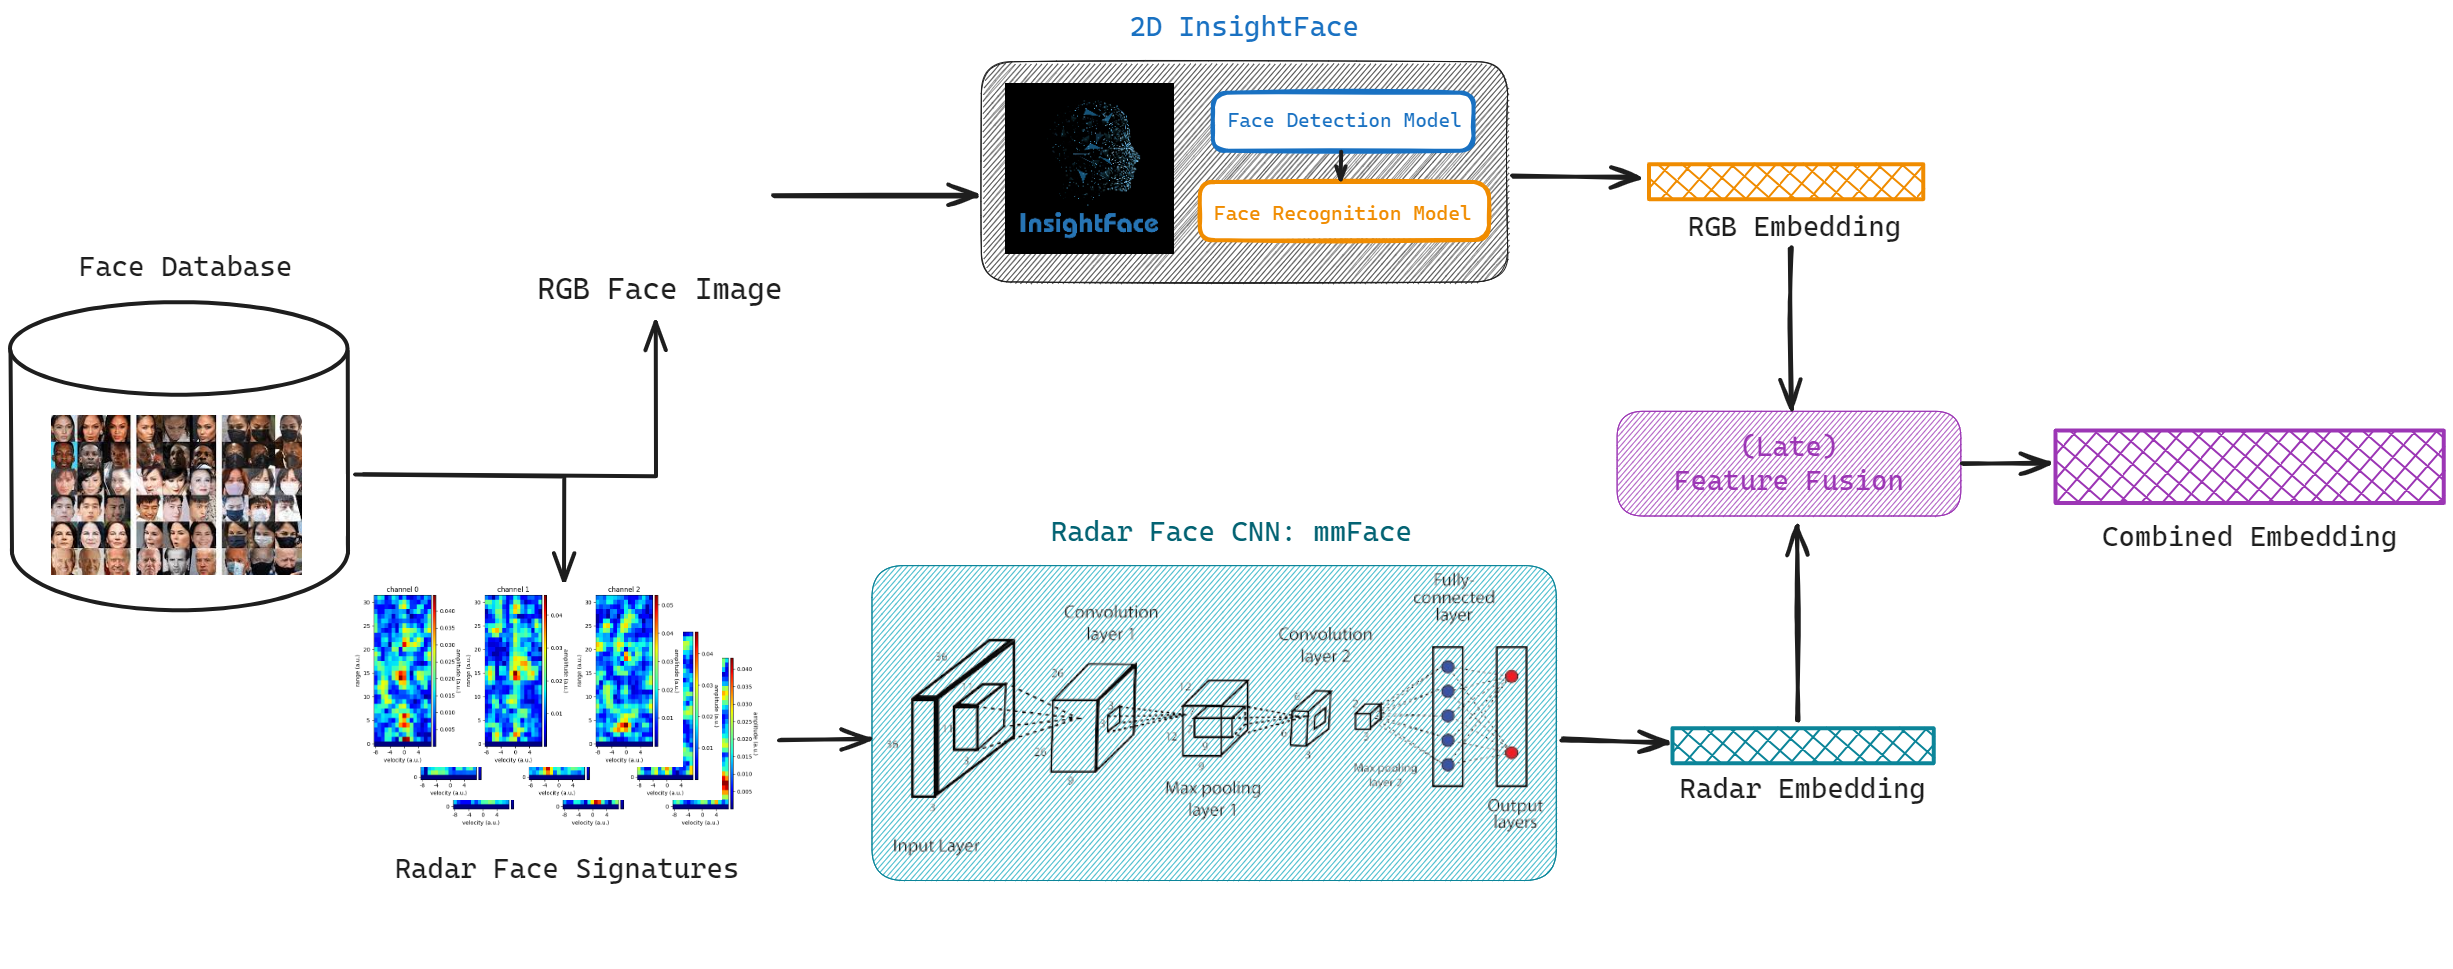
\includegraphics[width=0.8\textwidth]{images/model_architecture.png}
    \caption{High-level Model Architecture}
    \label{fig:model_architecture}
\end{figure}

Our proposed model will be built using a CNN-based architecture since it works best with image-like data. The Radar bursts from the data collection phase will be transformed into a Complex Range Doppler (CRD) map \cite{lien2016soli, hayashi2021radarnet} prior to feeding it into the model. Using the short-range configuration of the Google Soli at a centre frequency of 60 GHz with a maximum bandwidth of 5.5 GHz. Bursts are sampled at 25 Hz. The Intel RealSense is set to capture RGB-D frames at a sampling rate of 30 frames per second (FPS). Due to the difference in sampling rates between the two sensors, timestamps information is stored for the possibility of synchronising the two modalities for early data fusion.

As explained before, the data fusion techniques that will be explored are late-intermediate fusion and late, decision-level fusion. Purely intermediate feature-level fusion is not feasible due to the black-box treatment of the InsightFace model making it difficult to integrate features from both modalities in intermediary layers. However, a late feature-level fusion is possible combining the outputs of the last layers of each model to form an embedding combining both the RGB and mmFace features. Similarly, decision-level fusion will be explored since this involves mixing the predictions from the individual models. Early, data-level fusion would be the hardest to perform due to the dissimilarities between the two modalities in sampling rate and data format. The CRD maps must be synchronised and transformed into a depth image-like format before combining with the RGB images. Furthermore, this would require a whole new training cycle with the mmFace model which may be infeasible within the timeframe of the project. If time is available, then this will be looked at.

The dataset will be split by subjects into 80\%/10\%/10\% for training, validating and testing. This is due to the small size of the dataset of 50 subjects requiring a higher number of training samples for the mmFace model to learn effectively from. Following training, the testing phase will evaluate the distinctiveness of the output embeddings for distinct individuals. For accurate classifications, the individual faces must be spatial separable in the embedding space in order to discretely identify a person's face without ambiguity. t-SNE visualisations \cite{van2008visualizing} of the higher dimensional embeddings will also be employed to ensure this is the case to compare and contrast the attempting to classify the original data compared to with the output mappings. In addition, standard classification accuracies will be calculated to verify the identity recognition capabilities using the model against randomly selected ground truths. This will also allow comparisons with the results obtained from previous work with Radar-based 3D facial recognition.


\subsection{Progress}


%%%%%%%%%%%%%%%%%%%%%%%%%%%%%%%%%%%%%%%%%%%%%%%%%%%%%%%%%%%%%%%%%%%
\section{Work Plan}
show how you plan to organize your work, identifying intermediate deliverables and dates.

%%%%%%%%%%%%%%%%%%%%%%%%%%%%%%%%%%%%%%%%%%%%%%%%%%%%%%%%%%%%%%%%%%%
% it is fine to change the bibliography style if you want
\bibliographystyle{unsrt}
\bibliography{interim}
\end{document}
